
%%%%%%%%%%%%%%%%%%%%%%%%%%%%%%%%%%%%%%%%%%%%
\section{Introduction}

\begin{frame}
  \frametitle{Table of Contents}
  \tableofcontents[currentsection]
\end{frame}



\subsection{Clinical background}

%%%%%%%%%%%%%%%%%%%%%%%%%%%%%%%%%%%%%%%%%%%%%%%%%%%%%%%%
{
\paper{
ZUKETANG-Laparoscope-Laparoscopic-Simulator-Instruments;
Simendo simulator;
Laparo Analytic;
Gustavo A. Alonso-Silverio et al. in Surgical Education: Training for the Future 2018.
}

\begin{frame}{Training Surgical Skills}
      \begin{figure}
        \centering
        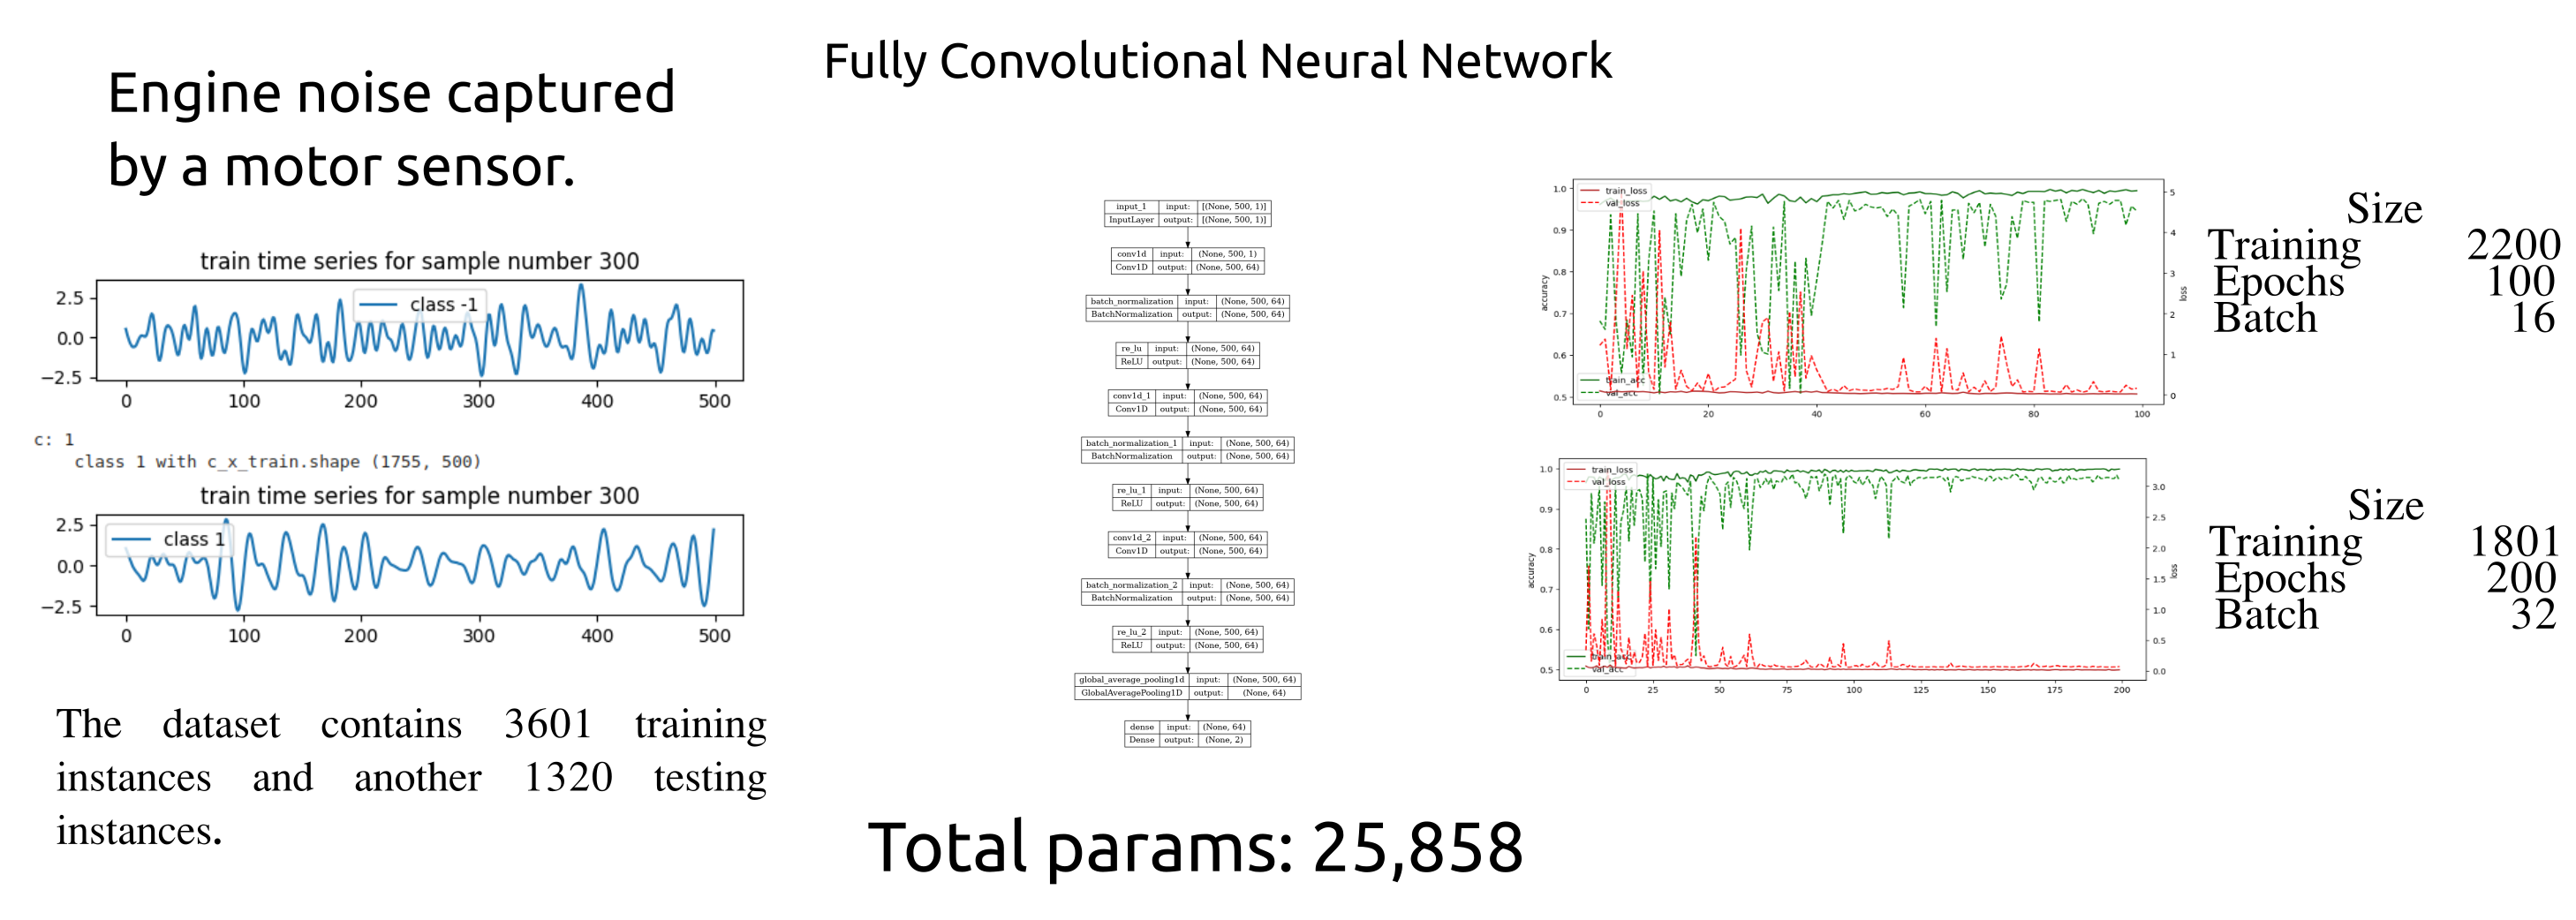
\includegraphics[width=1.0\textwidth]{main/outputs/drawing-v00.png}
        % \caption{The sonographer-probe-patient control system}
      \end{figure}
\end{frame}
}


\subsection{Research aims}
%%%%%%%%%%%%%%%%%%%%%%%%%%%%%%%%%%%%%%%%%%%%%%%%%%%%%%%%
{
%\paper{Wright-Gilbertson M. 2014 in PhD thesis}
\begin{frame}{Research aims}
\begin{itemize}
\item Design of reproducible workflow for data collection using multimodal sensors (e.g., USB video image and Bluetooth-based inertial sensors)
\item Investigate DL models with small memory and parameter size to enhance inference speed for surgical applications
% \item
\end{itemize}

\end{frame}
}

